\documentclass[10pt,twocolumn]{article}

\usepackage[margin=0.85in]{geometry}
\usepackage{amsmath,amssymb}
\usepackage{booktabs}
\usepackage{microtype}
\usepackage{xcolor}
\usepackage{tikz}
\usepackage{pgfplots}
\pgfplotsset{compat=1.16}
\usetikzlibrary{arrows.meta,positioning,shapes.geometric,backgrounds,fit,calc}
\usepackage[hidelinks]{hyperref}
\usepackage{pifont}
\usepackage{caption}
\captionsetup{font=small,labelfont=bf}

% palette (shared with the pillar-UDP congestion/redundancy papers)
\definecolor{pgood}{RGB}{31,119,80}
\definecolor{pbad}{RGB}{200,40,40}
\definecolor{pnode}{RGB}{38,70,120}
\definecolor{pcell}{RGB}{235,240,248}
\definecolor{pcellb}{RGB}{240,247,240}
\definecolor{pgray}{RGB}{110,110,110}
\definecolor{pmid}{RGB}{210,140,20}

\newcommand{\code}[1]{\texttt{\small #1}}
\newcommand{\Ks}{\ensuremath{K_s}}

\tikzset{
  node/.style={circle,draw=pnode,thick,fill=white,minimum size=6.5mm,
               font=\scriptsize\bfseries,inner sep=0pt},
  client/.style={rectangle,rounded corners=1pt,draw=black,thick,fill=white,
                 minimum height=7mm,minimum width=11mm,font=\scriptsize\bfseries},
  ingress/.style={rectangle,rounded corners=1.5pt,draw=pnode,thick,fill=white,
                  align=center,font=\tiny,inner sep=2pt,minimum width=22mm},
  db/.style={cylinder,shape border rotate=90,draw=pnode,fill=pcell,
             aspect=0.35,minimum height=9mm,minimum width=9mm,
             font=\tiny,align=center,inner sep=1pt},
  good/.style={-{Stealth[length=2mm]},pgood,thick},
  goodr/.style={-{Stealth[length=2mm]},pgood,thick,dashed},
  bad/.style={-{Stealth[length=2mm]},pbad,thick,dash pattern=on 1pt off 1.4pt},
  info/.style={-{Stealth[length=1.6mm]},pgray,semithick},
  rev/.style={-{Stealth[length=2mm]},pbad,thick},
}

\title{\vspace{-3.5em}\bfseries pillar-UDP: The Portable Cell-Minted Session Key
--- Transport-Frame Encryption without a Handshake}
\author{\normalsize pillar engineering \quad(machine-checked design note)}
\date{\normalsize 2026-09-09}

\begin{document}
\maketitle

\begin{abstract}
\noindent
pillar-UDP is a bare datagram substrate with no built-in cryptography, whose
posture is \emph{redundant datagrams sprayed across multiple paths, deduplicated
by content address, processed once}, served by ingress nodes that fail over and
load-balance (companion paper on congestion). A connection-oriented transport
handshake---libp2p Noise, or a per-pair WireGuard-style session---fights that
posture: its ordered multi-message exchange needs a reliability sublayer just to
land over lossy, unordered UDP, and it binds a session to \emph{one pair} of
endpoints, so a redundant copy that arrives at a different node, or an ingress
failover, cannot be served without re-handshaking. We instead treat the
\emph{cell} as a key-distribution centre. A client picks a fresh ephemeral
X25519 key; the transport session key
\Ks{}${}=\mathrm{HKDF}(\mathrm{ECDH}(\mathit{eph},\mathit{cell\_static}),
\mathit{nonce})$ is \emph{deterministically} derived, so the client and
\emph{every} cell node compute the byte-identical \Ks{} with no round-trip and no
race. The authorization is a \emph{cell-signed record on streamdb} that converges
cell-wide; \Ks{} is never stored, only its derivation inputs, and any node
recomputes it---making the session \emph{portable} across every node (ingress
failover, relay, load-balancing). Sender identity comes from the ed25519
signature inside the \code{PillarMessage}, not from \Ks{} (which only proves cell
membership); replay defence is the content-addressed dedup pillar already runs;
forward secrecy is deliberately bounded to cell-key security plus a
\emph{security-critical} erase-on-revoke. Anonymity is a \emph{policy} state, not
a separate crypto path: an anonymous key runs the identical flow and is confined
by default-deny WoT/RBAC. The design is machine-checked in TLA\textsuperscript{+}
(\code{PillarUdpEncryption.tla}, green under TLC before any Rust): the session
converges on one cell-signed key, a node serves only an authorized session,
replay is idempotent, an unattested principal never gains a privileged grant, and
a revoked key is eventually erased. This scheme applies \emph{only} to pillar-UDP;
QUIC and TCP fall back to their own TLS 1.3.
\end{abstract}

\section{Why not Noise, and why not a per-pair session}
Two candidate transport-crypto designs were rejected against pillar-UDP's
multipath, any-ingress posture.

\textbf{libp2p Noise upgrade} is a \emph{session/connection} protocol. Its
handshake is a strict ordered multi-message exchange that needs a reliability
sublayer just to land over lossy, unordered UDP, and it binds a session to
\emph{one pair} of endpoints. That fights the connectionless, multipath,
any-ingress model.

\textbf{A per-pair Noise/WireGuard session} gives forward secrecy and replay
protection, but a session bound to a pair is \emph{not portable}: if the first
ingress node dies, or a redundant copy arrives at a different node, the session
cannot be served without re-handshaking.

The blocker to portability is precise and cryptographic. An AEAD session is
\emph{a shared key plus a per-direction monotonic nonce counter}. The \emph{key}
is portable; the \emph{counter} is not---two nodes incrementing one counter would
reuse a nonce, and AEAD nonce reuse is a total break (keystream reuse
$\Rightarrow$ plaintext recovery; authentication-key leak $\Rightarrow$ forgery).
Remove the shared counter and derive the nonce collision-free instead---convergent
(\code{HKDF(\Ks, content\_address(frame))}) or sender-partitioned
(\code{node\_id\,\(\|\)\,counter})---and the key becomes portable across every node
that holds it. That is the whole idea.

\section{The scheme: the cell is a KDC, the session key rides streamdb}
pillar already has a shared trust boundary (the \emph{cell}, a genesis principal
with a static key), a converging cell-internal state substrate (\emph{streamdb}),
per-message \emph{ed25519 signatures}, and \emph{content-addressed dedup}---exactly
the ingredients a portable session needs. So the transport session key is built
from them: it is portable and cell-scoped (every node can derive and serve it, no
per-pair binding); it is \emph{deterministically derived}, not
minted-and-reconciled (two ingress nodes handling the same sprayed init derive the
byte-identical key---no race); it is \emph{authorized by a cell-signed streamdb
record} that converges to every node (so failover / relay / load-balancing all
serve one session); and anonymity is a policy state, not a separate scheme
(\S\ref{sec:anon}). The end-to-end exchange is drawn in Fig.~\ref{fig:flow}
and as a time sequence in Fig.~\ref{fig:seq}.

\subsection{Key derivation (deterministic, portable)}
A client---a node, a non-node client, or an anonymous client---opens a session by
choosing a fresh ephemeral X25519 keypair $(\mathit{eph\_pk},\mathit{eph\_sk})$
and a random \code{client\_nonce}. The session key is a static-ephemeral ECDH
against the cell static key, run through an HKDF with a domain separator distinct
from the content seal:
\begin{align*}
\mathit{shared} &= \mathrm{X25519}(\mathit{eph\_sk},\ \mathit{cell\_static\_pk})\\[-1pt]
   &= \mathrm{X25519}(\mathit{cell\_static\_sk},\ \mathit{eph\_pk})\\
\Ks &= \mathrm{HKDF}(\mathit{shared},\ \text{salt}{=}\mathit{client\_nonce},\\[-1pt]
    &\hphantom{{}={}} \text{info}{=}\text{``pillar-udp/session/v1''})\\
\mathit{sid} &= \mathrm{addr}(\mathit{eph\_pk}\,\|\,\mathit{client\_nonce})
\end{align*}
The first line is the client's derivation, the second any cell node's---equal by
the Diffie--Hellman symmetry, so no key crosses the wire.
Both endpoints compute the \emph{same} \Ks{} with no key on the wire and no
round-trip: the client derives it the instant it picks $\mathit{eph\_pk}$ (it
knows the published $\mathit{cell\_static\_pk}$); \emph{every} cell node derives
the identical \Ks{} from $(\mathit{cell\_static\_sk},\mathit{eph\_pk},
\mathit{client\_nonce})$ carried in the session record. Because \Ks{} is a pure
function of those inputs, two racing ingress nodes cannot diverge---the
``collision'' is byte-identical, so there is nothing for the client to reject.
\Ks{} is \emph{never at rest}: streamdb stores only the derivation inputs plus the
cell authorization, and any node recomputes \Ks{} on demand. Per-datagram AEAD
nonces under \Ks{} are collision-free without coordination (convergent or
sender-partitioned), so the many cell nodes sharing \Ks{} never reuse a nonce.

\subsection{The session record (cell-signed, on streamdb)}
The record carries no key material---only the inputs from which \Ks{} is derivable
by a cell-secret holder, plus the cell signature that any node verifies before
honoring the session:
\begin{quote}\scriptsize\ttfamily
SessionRecord \{\\
\hspace*{1.2em}session\_id\ \ : Cid\ // addr(eph\_pk\(\|\)nonce)\\
\hspace*{1.2em}principal\_pk : PublicKey // node/user/anon\\
\hspace*{1.2em}eph\_pk\ \ \ \ \ : X25519PublicKey\\
\hspace*{1.2em}client\_nonce : bytes\\
\hspace*{1.2em}grants\ \ \ \ \ : PolicySet // WoT/RBAC \S\ref{sec:anon}\\
\hspace*{1.2em}not\_after\ \ \ : Timestamp\\
\hspace*{1.2em}cell\_sig\ \ \ \ : Signature // signed by CELL key\\
\}
\end{quote}
streamdb convergence makes the record available cell-wide.

\begin{figure*}[t]
\centering
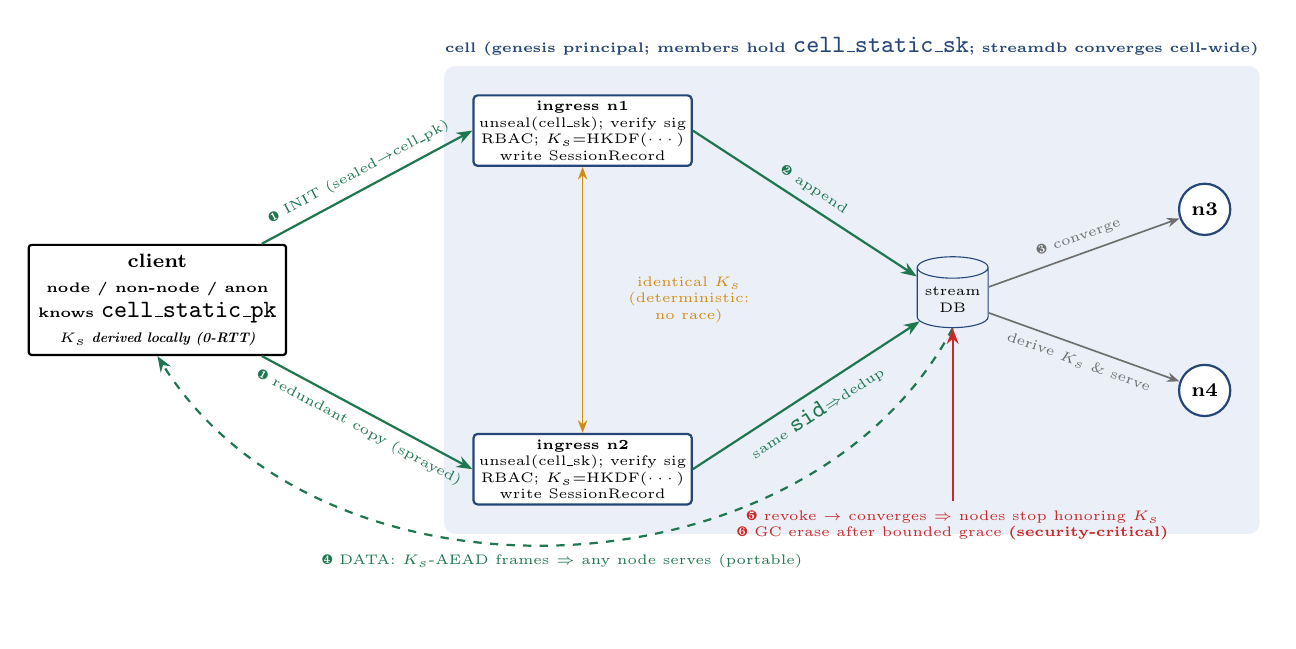
\begin{tikzpicture}[node distance=6mm]
  % client (left, outside the cell)
  \node[client,align=center] (c) at (0,0)
     {client\\[1pt]{\tiny node / non-node / anon}\\[1pt]
      {\tiny knows \code{cell\_static\_pk}}\\[1pt]
      {\tiny\itshape \Ks{} derived locally (0-RTT)}};
  % ingress nodes (well separated vertically)
  \node[ingress] (n1) at (5.4, 2.15)
     {\textbf{ingress n1}\\ unseal(cell\_sk); verify sig\\ RBAC; \Ks{}=HKDF($\cdots$)\\ write SessionRecord};
  \node[ingress] (n2) at (5.4,-2.15)
     {\textbf{ingress n2}\\ unseal(cell\_sk); verify sig\\ RBAC; \Ks{}=HKDF($\cdots$)\\ write SessionRecord};
  % streamdb + other cell nodes
  \node[db] (db) at (10.1, 0.0) {stream\\DB};
  \node[node] (n3) at (13.3, 1.15) {n3};
  \node[node] (n4) at (13.3,-1.15) {n4};
  % cell backdrop
  \begin{scope}[on background layer]
    \node[fill=pcell,rounded corners,fit=(n1)(n2)(db)(n3)(n4),
          inner sep=3.6mm,label={[font=\tiny\bfseries,pnode]above:cell
          (genesis principal; members hold \code{cell\_static\_sk}; streamdb
          converges cell-wide)}] {};
  \end{scope}
  % (1) INIT sprayed, redundant, multipath
  \draw[good] (c) -- node[above,font=\tiny,pgood,sloped]{\ding{182} INIT (sealed$\to$cell\_pk)} (n1.west);
  \draw[good] (c) -- node[below,font=\tiny,pgood,sloped]{\ding{182} redundant copy (sprayed)} (n2.west);
  % identical Ks between the two ingress -- label parked in open space to the right
  \draw[{Stealth[length=1.6mm]}-{Stealth[length=1.6mm]},pmid,semithick] (n1.south) -- (n2.north);
  \node[font=\tiny,pmid,align=center,fill=pcell,inner sep=1pt] at (6.75,0)
       {identical \Ks{}\\(deterministic:\\no race)};
  % (2) append to streamdb -> dedup
  \draw[good] (n1.east) -- node[above,font=\tiny,pgood,sloped]{\ding{183} append} (db);
  \draw[good] (n2.east) -- node[below,font=\tiny,pgood,sloped]{same \code{sid}$\Rightarrow$dedup} (db);
  % (3) replicate to other nodes
  \draw[info] (db) -- node[above,font=\tiny,pgray,sloped]{\ding{184} converge} (n3);
  \draw[info] (db) -- node[below,font=\tiny,pgray,sloped]{derive \Ks{} \& serve} (n4);
  % (4) DATA reply: dashed arc dipping well BELOW the ingress row, back to client
  \draw[goodr] (db.south) to[bend left=60]
     node[below,font=\tiny,pgood,pos=0.5]
        {\ding{185} DATA: \Ks{}-AEAD frames $\Rightarrow$ any node serves (portable)}
     (c.south);
  % (5)(6) revoke + GC: compact tag hanging under the store, red arrow up
  \node[font=\tiny,pbad,align=center,anchor=north] (rv) at (10.1,-2.55)
     {\ding{186} revoke $\to$ converges $\Rightarrow$ nodes stop honoring \Ks{}\\
      \ding{187} GC erase after bounded grace \textbf{(security-critical)}};
  \draw[rev] (rv.north) -- (db);
\end{tikzpicture}
\caption{\textbf{Packet flow.} \ding{182}~The client sprays a cell-sealed init
(fresh ephemeral $+$ nonce) over redundant paths; either or both ingress nodes
process it and, because \Ks{} is a deterministic function of
$(\mathit{cell\_sk},\mathit{eph\_pk},\mathit{nonce})$, derive the
\emph{byte-identical} key. \ding{183}~Each writes a cell-signed
\code{SessionRecord}; identical \code{session\_id} means the store dedups to one
record. \ding{184}~streamdb converges the record cell-wide, so nodes \code{n3},
\code{n4} can now derive \Ks{} and serve the session. \ding{185}~Data frames are
\Ks{}-AEAD-sealed with a convergent nonce and carry an inner \code{PillarMessage}
signed by the client's key (sender identity); any node holding the record serves
them, and a replayed frame has the same Cid and is deduped. \ding{186}~On
close/timeout a cell-signed revocation converges and every node stops honoring
\Ks{}. \ding{187}~GC erasing the record is a \emph{security} operation, not
hygiene. A non-node client and an anonymous client run the identical flow; only
the RBAC outcome differs (\S\ref{sec:anon}). Modeled in
\code{PillarUdpEncryption.tla}.}
\label{fig:flow}
\end{figure*}

\begin{figure*}[t]
\centering
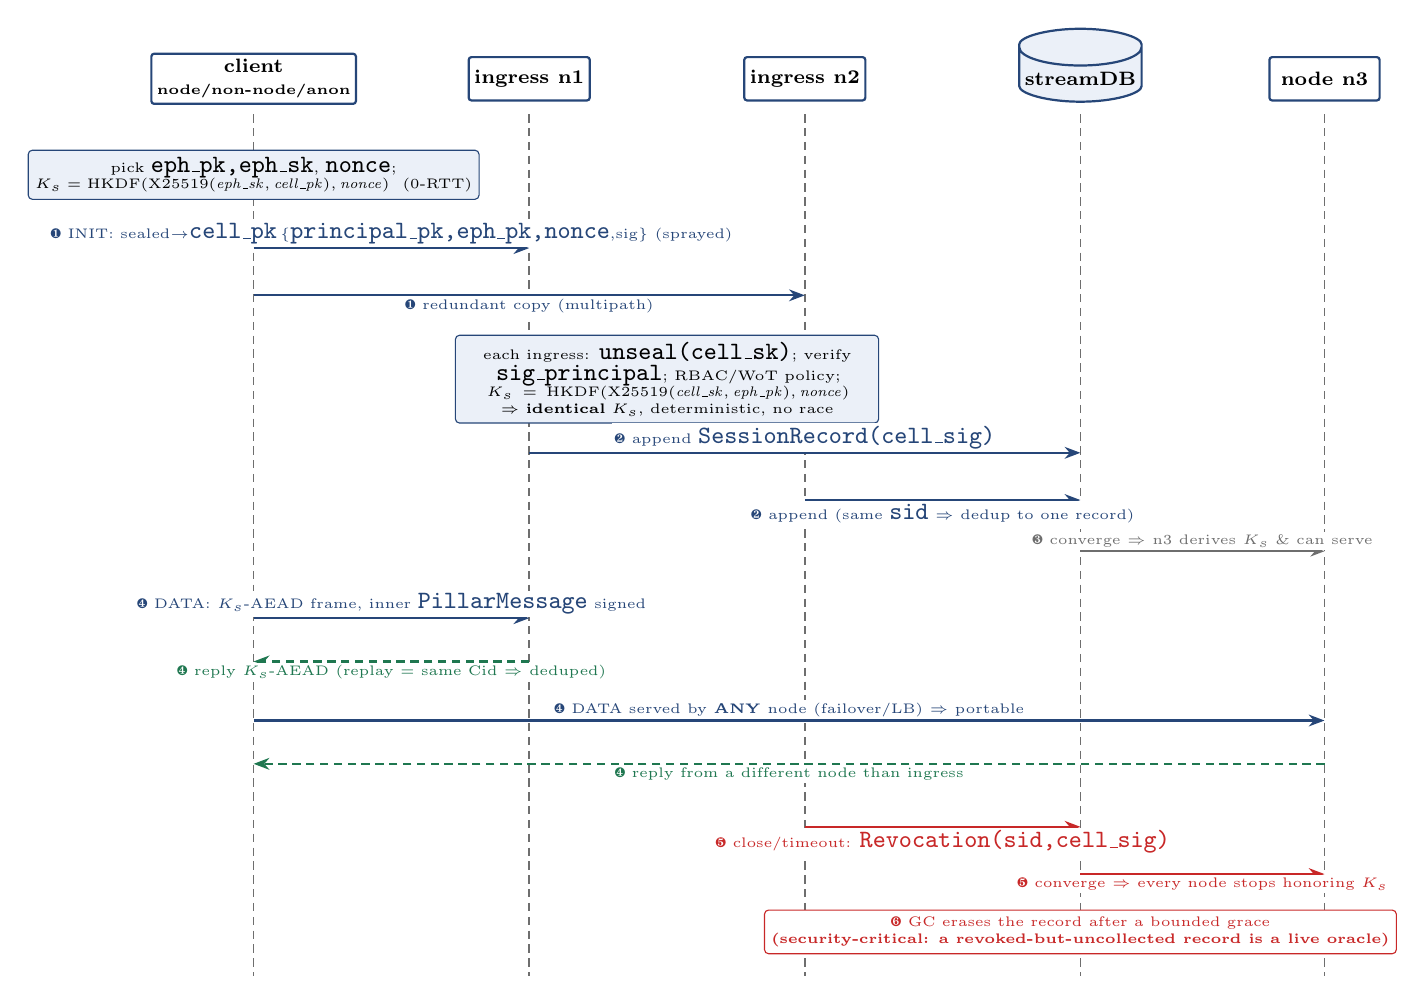
\begin{tikzpicture}[
  part/.style={rectangle,rounded corners=1pt,draw=pnode,thick,fill=white,
               font=\scriptsize\bfseries,minimum height=5.5mm,minimum width=14mm,
               align=center,inner sep=2pt},
  life/.style={pgray,densely dashed,semithick},
  msg/.style={-{Stealth[length=2mm]},thick,pnode},
  ret/.style={-{Stealth[length=2mm]},thick,pgood,densely dashed},
  rev/.style={-{Stealth[length=2mm]},thick,pbad},
  cvg/.style={-{Stealth[length=1.8mm]},semithick,pgray},
  lbl/.style={midway,above,font=\tiny,fill=white,inner sep=1pt},
  lblb/.style={midway,below,font=\tiny,fill=white,inner sep=1pt},
  note/.style={rectangle,rounded corners=1.5pt,draw=pnode,fill=pcell,
               font=\tiny,align=center,inner sep=2.5pt},
  act/.style={rectangle,draw=pnode,fill=pcell,minimum width=1.7mm}]
  % ---- lifelines (x positions) ----
  \def\xC{0}    \def\xA{3.5}  \def\xB{7.0}  \def\xD{10.5} \def\xE{13.6}
  \def\ybot{-11.4}
  \foreach \x in {\xC,\xA,\xB,\xD,\xE}
     \draw[life] (\x,-0.45) -- (\x,\ybot);
  % ---- participant headers ----
  \node[part] at (\xC,0) {client\\{\tiny node/non-node/anon}};
  \node[part] at (\xA,0) {ingress n1};
  \node[part] at (\xB,0) {ingress n2};
  \node[part,shape=cylinder,shape border rotate=90,aspect=0.3,fill=pcell] at (\xD,0) {streamDB};
  \node[part] at (\xE,0) {node n3};
  % ---- messages, time flows downward ----
  \node[note,anchor=north] at (\xC,-0.9)
     {pick \code{eph\_pk,eph\_sk}, \code{nonce};\\
      $\Ks{}=\mathrm{HKDF}(\mathrm{X25519}(\mathit{eph\_sk},\mathit{cell\_pk}),\mathit{nonce})$ \ (0-RTT)};
  \draw[msg] (\xC,-2.15) -- node[lbl]{\ding{182} INIT: sealed$\to$\code{cell\_pk}\,\{\code{principal\_pk,eph\_pk,nonce},sig\} (sprayed)} (\xA,-2.15);
  \draw[msg] (\xC,-2.75) -- node[lblb]{\ding{182} redundant copy (multipath)} (\xB,-2.75);
  \node[note,anchor=north,text width=52mm] at ($(\xA,-3.25)!0.5!(\xB,-3.25)$)
     {each ingress: \code{unseal(cell\_sk)}; verify \code{sig\_principal}; RBAC/WoT policy;\\
      $\Ks{}=\mathrm{HKDF}(\mathrm{X25519}(\mathit{cell\_sk},\mathit{eph\_pk}),\mathit{nonce})$
      \ $\Rightarrow$ \textbf{identical \Ks{}}, deterministic, no race};
  \draw[msg] (\xA,-4.75) -- node[lbl]{\ding{183} append \code{SessionRecord(cell\_sig)}} (\xD,-4.75);
  \draw[msg] (\xB,-5.35) -- node[lblb]{\ding{183} append (same \code{sid} $\Rightarrow$ dedup to one record)} (\xD,-5.35);
  \draw[cvg] (\xD,-6.0) -- node[lbl]{\ding{184} converge $\Rightarrow$ n3 derives \Ks{} \& can serve} (\xE,-6.0);
  \draw[msg] (\xC,-6.85) -- node[lbl]{\ding{185} DATA: \Ks{}-AEAD frame, inner \code{PillarMessage} signed} (\xA,-6.85);
  \draw[ret] (\xA,-7.4) -- node[lblb]{\ding{185} reply \Ks{}-AEAD (replay = same Cid $\Rightarrow$ deduped)} (\xC,-7.4);
  \draw[msg] (\xC,-8.15) -- node[lbl]{\ding{185} DATA served by \textbf{ANY} node (failover/LB) $\Rightarrow$ portable} (\xE,-8.15);
  \draw[ret] (\xE,-8.7) -- node[lblb]{\ding{185} reply from a different node than ingress} (\xC,-8.7);
  \draw[rev] (\xB,-9.5) -- node[lblb]{\ding{186} close/timeout: \code{Revocation(sid,cell\_sig)}} (\xD,-9.5);
  \draw[rev] (\xD,-10.1) -- node[lblb]{\ding{186} converge $\Rightarrow$ every node stops honoring \Ks{}} (\xE,-10.1);
  \node[note,anchor=north,draw=pbad,fill=white] at (\xD,-10.55)
     {\color{pbad}\ding{187} GC erases the record after a bounded grace\\
      \color{pbad}\textbf{(security-critical: a revoked-but-uncollected record is a live oracle)}};
\end{tikzpicture}
\caption{\textbf{Time sequence.} The same flow as Fig.~\ref{fig:flow}, ordered in
time. The client derives \Ks{} locally the instant it picks its ephemeral (0-RTT),
then sprays the cell-sealed init over redundant paths. \emph{Both} ingress nodes
can process the init and, running the mirror-image ECDH against the cell static
key, derive the \emph{byte-identical} \Ks{}---so the two \code{SessionRecord}
appends carry the same \code{sid} and streamdb dedups them to one cell-signed
record. Convergence lets a node (\code{n3}) that never saw the init derive \Ks{}
and serve the session, which is why data frames are portable: a reply may come
from a \emph{different} node than ingested the client. On close or timeout a
cell-signed revocation converges and every node stops honoring \Ks{}; GC then
erasing the record is a security operation, since a revoked-but-uncollected record
keeps \Ks{} derivable. An anonymous client follows the identical sequence---only
the RBAC policy outcome at each ingress differs (\S\ref{sec:anon}).}
\label{fig:seq}
\end{figure*}

\section{What each layer provides (and deliberately does not)}
\textbf{Confidentiality of framing}---\Ks{}-AEAD on every pillar-UDP datagram.
(Application content is \emph{additionally} cell-sealed end-to-end,
\code{pillar-message-format} \S5.) \textbf{Sender identity}---\emph{not} from \Ks{}
(which only proves cell membership, since every node holds it) but from the
ed25519 signature inside the \code{PillarMessage}; the transport key gives
group-level confidentiality, identity is a content-layer property.
\textbf{Replay protection}---from content-addressed dedup: a replayed datagram has
the same Cid and is dropped by the store pillar already runs; no per-session replay
window is needed. \textbf{Portability / failover / load-balancing}---any node with
the converged record derives the same \Ks{} and serves the session.
\textbf{Forward secrecy}---bounded to cell-key security plus erase-on-revoke,
\emph{by design}. \Ks{} is derivable under the cell static key, so a cell-key
compromise exposes past sessions; this is the identical tradeoff the content
cell-seal already accepts. FS \emph{independent} of the cell key would require a
discarded ephemeral DH secret, which directly contradicts a portable,
cell-derivable key---so it is deliberately traded for cross-node portability.
Mitigations: periodic cell rekey, and erase on revoke.

\section{Revocation and GC are security-critical}
On close or timeout a cell node writes a cell-signed \emph{revocation} for the
\code{session\_id} to streamdb; convergence stops every node from honoring \Ks{}.
GC of the revoked record is a \emph{security operation, not hygiene}: a
revoked-but-uncollected record keeps \Ks{} derivable, i.e.\ a live decryption
oracle for any captured ciphertext, so GC must erase within a bounded deadline.
Ciphertext captured \emph{before} revocation stays readable by anyone who held
\Ks{}---inherent to shared-key transport and accepted.

\section{Anonymous sessions {=} the same scheme {+} policy}
\label{sec:anon}
An anonymous client generates an anonymous signing key and runs the \emph{exact
scheme} of \S2 and Fig.~\ref{fig:flow}. The anonymous key is \emph{cryptographically
equivalent} to a user or node key and is subject to the \emph{same WoT/RBAC checks}
as any principal. The only difference is the \emph{policy outcome}: absent signed
role attestations for the key, the cell's default-deny RBAC withholds sensitive
data and privileged operations---the anonymous session can communicate, but only
within an unattested principal's grant set. Nothing else about key derivation,
portability, revocation, or nonce discipline changes. Two consequences:
\emph{anonymous $\Rightarrow$ pseudonymous, not automatically unlinkable}---a
stable anonymous key lets the cell link a client across sessions, so unlinkability
is a client choice (fresh key, hence fresh \code{session\_id}, per session); and
\emph{the policy gate is the whole security boundary for anonymity}---it rests on
the ROI invariant that every controller enforces WoT/RBAC default-deny, so an
unattested principal must never acquire a privileged grant.

\section{Compatibility \& rollout}
Dropping the libp2p Noise upgrade is a \emph{breaking} pillar-UDP change, gated by
the versioning spine: the pillar-UDP protocol version bumps and compatibility
negotiation refuses a legacy-Noise peer cleanly rather than mis-framing. A mixed
legacy-Noise / session-key swarm must coexist through the rollout window
(\code{RollingCoexistence}, \code{NegotiationRefusesIncompatible} in the
message-format spec). QUIC/TCP peers are unaffected---they never used this path.

\section{Machine-checked obligations}
The design is TLA\textsuperscript{+}-gated (method \#1): \code{PillarUdpEncryption.tla}
must be green under TLC before any Rust. Table~\ref{tab:inv} lists the obligations;
all pass, together with the full specs gate and the schema round-trip.

\begin{table}[t]
\footnotesize
\setlength{\tabcolsep}{4pt}
\begin{tabular}{@{}p{0.34\columnwidth}p{0.60\columnwidth}@{}}
\toprule
\textbf{Invariant} & \textbf{Guarantee} \\
\midrule
\code{SessionKey\-CellSigned} & every honored session is backed by a cell-signed record \\
\code{SessionConvergesOn\-OneKey} & $\le 1$ active authorization per \code{session\_id}; every node derives the identical \Ks{} the client did \\
\code{SessionAuthorized\-BeforeServe} & a node serves only a session it has actually converged (no fabricated/unauthorized sessions) \\
\code{AnonIsUnattested\-Principal} & a principal with no attestations holds only the restricted grant; never a privileged one \\
\code{SharedKeyReplay\-ViaDedup} & applying a frame is content-addressed \& idempotent; a replay causes no second effect \\
\code{RevokedKeyEventual\-lyErased} \emph{(liveness)} & a revoked session's record is eventually erased from streamdb and every node's view \\
\code{NonceCollisionFree} & the per-frame nonce under \Ks{} is injective in the plaintext (AEAD safety); discharged as a constant assumption \\
\bottomrule
\end{tabular}
\caption{TLA\textsuperscript{+} obligations of \code{PillarUdpEncryption.tla}.
Forward secrecy is a \emph{documented, accepted} property (\S4), not a state
invariant: it is a statement about a hypothetical cell-key compromise,
deliberately bounded rather than proven absent.}
\label{tab:inv}
\end{table}

% flush the pending double-column float (Fig 2) and Table 1 so they precede this section
\clearpage
\section{Relationship to the content seal}
Independent layers, composed. The \emph{content seal} (\code{pillar-message-format}
\S5) is end-to-end to the cell, convergent, transport-agnostic, and gives the
stable Cid. The \emph{transport frame seal} (this paper) is pillar-UDP-specific,
keyed by the portable session key, and protects on-wire framing. A pillar-UDP
datagram carries a cell-sealed body inside a session-key-sealed frame; on QUIC/TCP
the outer frame seal is the transport's TLS instead, and the content seal is
unchanged.

\begin{thebibliography}{9}
\bibitem{noise} T.~Perrin, \emph{The Noise Protocol Framework}, Rev.~34, 2018.
\bibitem{wireguard} J.~A.~Donenfeld, \emph{WireGuard: Next Generation Kernel
  Network Tunnel}, NDSS, 2017.
\bibitem{hkdf} H.~Krawczyk, \emph{Cryptographic Extraction and Key Derivation:
  The HKDF Scheme}, CRYPTO, 2010.
\bibitem{tlaplus} L.~Lamport, \emph{Specifying Systems}, Addison-Wesley, 2002.
\end{thebibliography}

\end{document}
